% 2D Image with indices
% Author: Peter Steinbach
\documentclass[tikz]{standalone}
%\documentclass[dvisvgm]{standalone}
%\def\pgfsysdriver{pgfsys-tex4ht.def}
\usepackage{tikz}
\usetikzlibrary{calc,trees,positioning,arrows.meta,chains,shapes.geometric,shapes.arrows,%
    decorations.pathreplacing,decorations.pathmorphing,shapes,%
    matrix,shapes.symbols,fit,backgrounds}

 \pgfdeclarelayer{back}
 \pgfsetlayers{background,back,main}


\makeatletter
\makeatother

\begin{document}
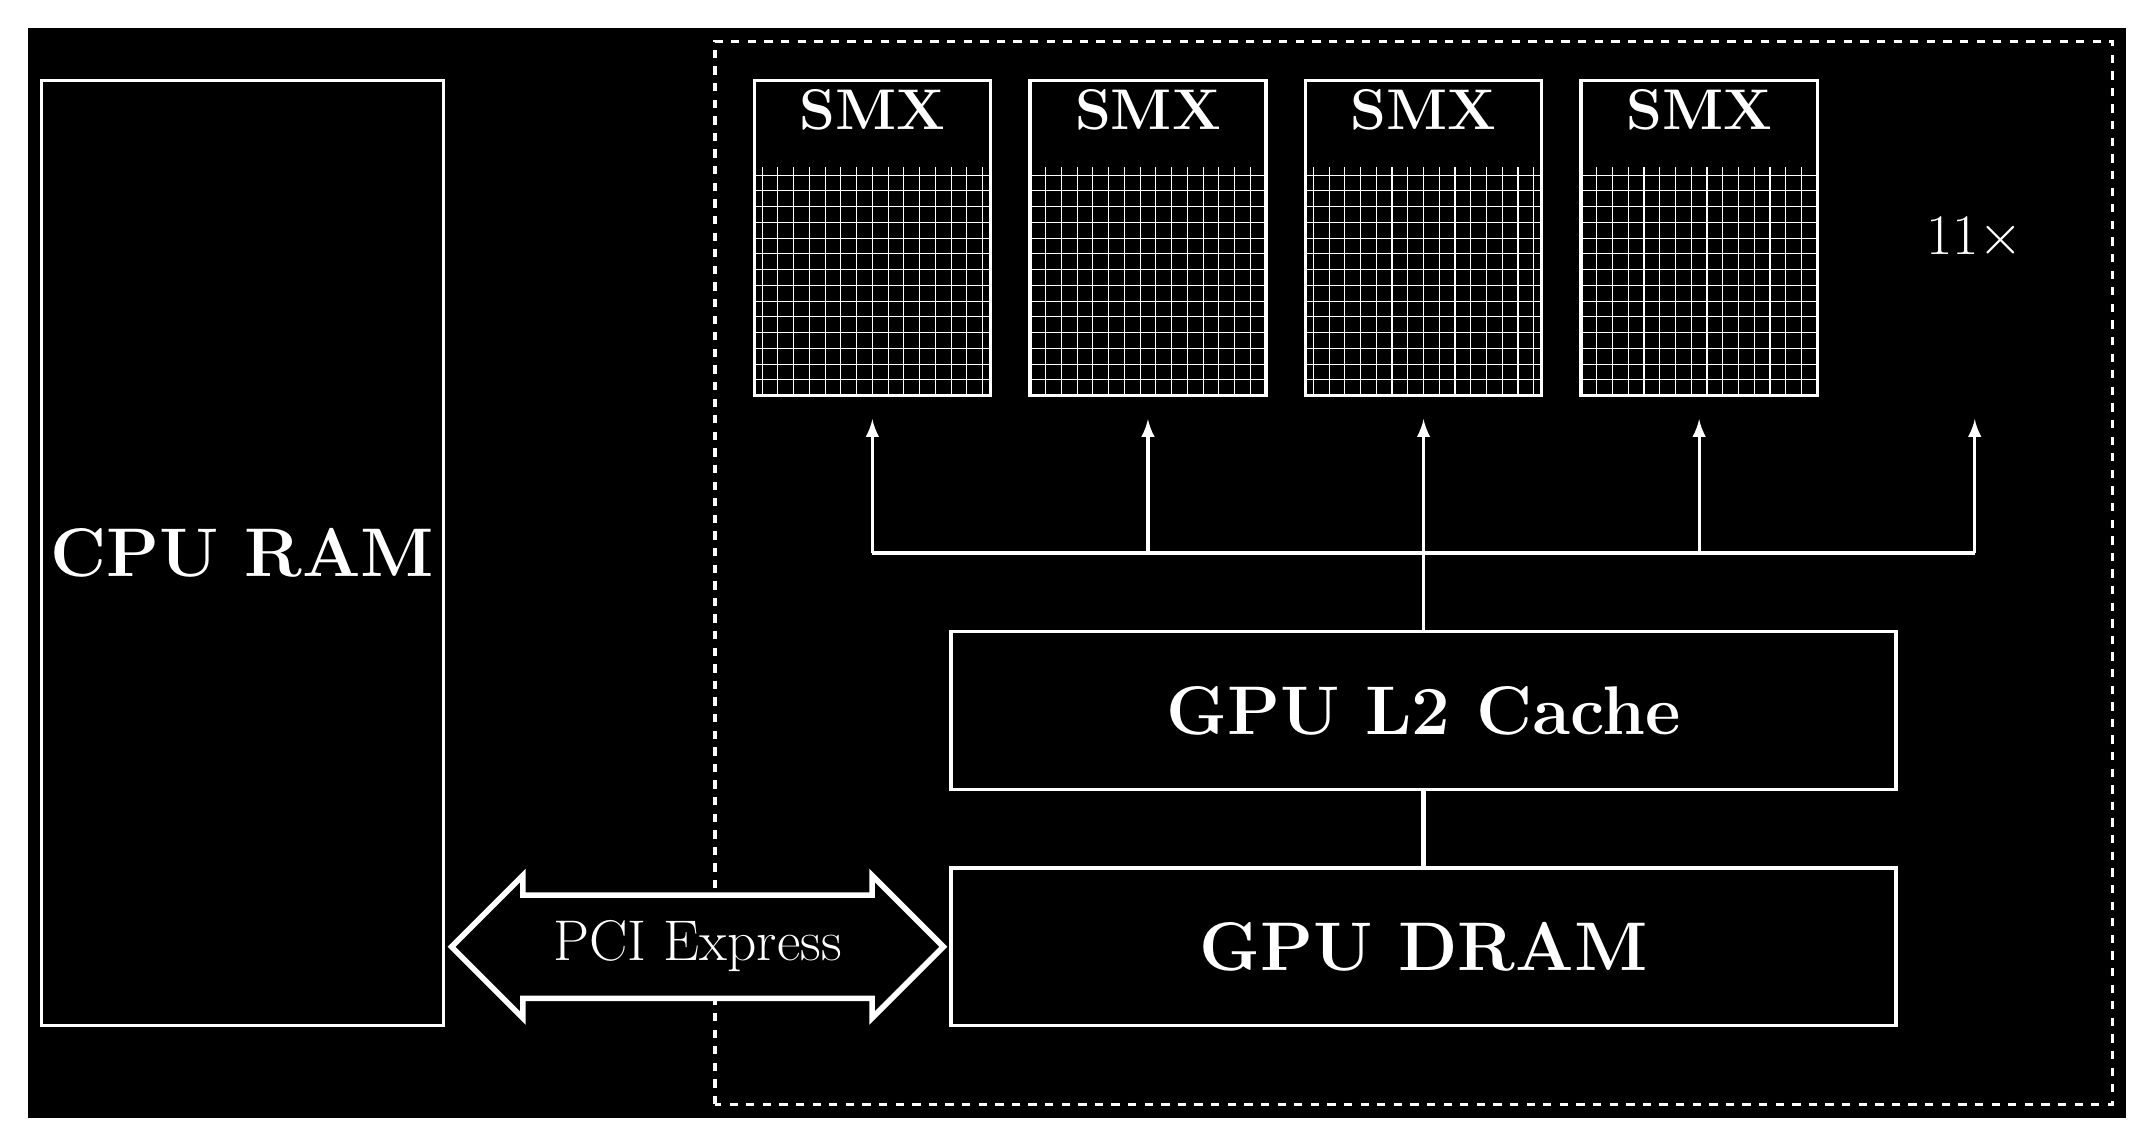
\begin{tikzpicture}[
  show background rectangle, 
  background rectangle/.style={fill=black},
  color=white,
  help lines/.style={color=lightgray,line width=.2pt},
  ]

%  \draw[dashed, very thick] (5,-1) rectangle (25,14) ;
  \foreach \c in {0,...,3}
  {
    %\draw[-] ($(0.2,2.05)+(2.4*\c,0)$) rectangle ($(2.3,2.75)+(2.4*\c,0)$) node[fitting node] (l2_\c) {\bfseries{}L2};
    \node (smx_\c) [very thick,draw,rectangle, minimum width=3cm, minimum height=4cm,font=\huge] at($(8,10)+(3.5*\c,0)$) {};
    \node [very thick,font=\huge,anchor=north] at(smx_\c.north) {\bfseries{}SMX};
    \node (smx_\c_topright) [below =of smx_\c.north east] {};
    \draw[step=.2] (smx_\c.south west) grid (smx_\c_topright);
  }



  \foreach \i in {0,...,4}
  \draw[-latex,very thick] ($(8,6)+(3.5*\i,0)$) -- ($(8,7.7)+(3.5*\i,0)$) 
  ;
  
  \node (dots) [text=white,font=\huge] at($(8,10)+(14,0)$) {\bfseries{}$11\times$};

  \draw[dashed,very thick] (6,-1) rectangle ($(dots)+(1.75,2.5)$);


  \draw[very thick] ($(8,6)$) -- ($(8,6)+(3.5*4,0)$) ;

  \node (l2cache) [very thick,draw,rectangle, minimum width=12cm, minimum height=2cm,font=\Huge] at($(8,10)+(7,-6)$) {\bfseries{}GPU L2 Cache};
  \node (dram) [very thick,draw,rectangle, minimum width=12cm, minimum height=2cm,font=\Huge] at($(8,10)+(7,-9)$) {\bfseries{}GPU DRAM};

  \node (cpu_ram) [very thick,draw,rectangle, minimum width=4.5cm, minimum height=12cm,font=\Huge] at($(0,10)+(0,-4)$) {\bfseries{}CPU RAM};

  % \draw[ultra thick] (cpu_ram) -- (dram);
  
  %\draw[|<->|,very thick,double equal sign distance, line width=1mm, double distance=1.5mm,-Stealth] (dram.west) -- (cpu_ram.east);
  \node (middle) at($(dram.west)+(-3.2,0)$) {};
  \node [double arrow, draw, fill=black,line width=2pt,font=\huge,inner xsep=.6cm,inner ysep=.3cm] at(middle) {PCI Express};
  \draw[ultra thick] (l2cache.south) -- (dram.north);


  \draw[very thick] (dram) -- (l2cache);
  \draw[very thick] (l2cache) -- ($(8,6)+(7,0)$);
  

\end{tikzpicture}
\end{document}
